\beginsong{Es soll sich der Mensch}[
    txt={nach den 'Hayner Dorfmusikanten'},
    txtjahr={um 1800},
    mel={Fiedel Michel},
    meljahr={1978}, 
    bo={130}, 
    pfii={82}, 
    pfiii={44}, 
    siru={76},
    tonspur={262}, 
]

\beginverse
\endverse
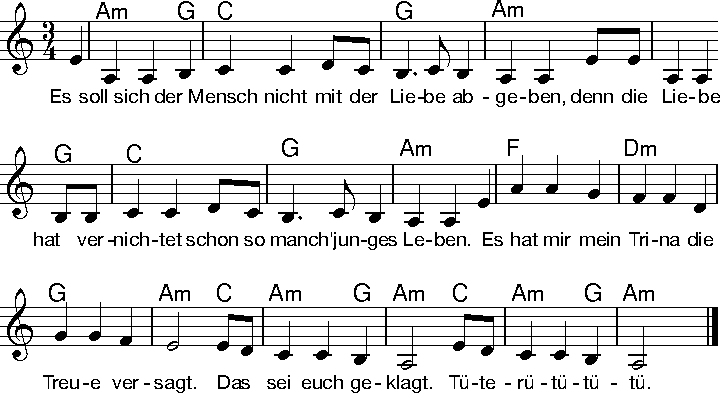
\includegraphics[draft=false, width=1\textwidth]{Noten/Lied039.pdf}	

\beginverse
Ich \[Am]war ja \[G]so \[C]schrecklich in die \[G]Trina ver\[Am]schossen;
mein Herz war \[G]mit \[C]Zucker und mit \[G]Honig über\[Am]gossen.
Da \[F]kommt doch, zum \[Dm]Teufel, dem \[G]Müller sein \[Am]Franz
\[C]und der \[Am]führt sie \[G]zum \[Am]Tanz. \[C]Tü-te-\[Am]rü-tü-\[G]tü-\[Am]tü.
\endverse

\beginverse
Und nun ^schmeckt mir ^kein ^Essen und es ^schmeckt mir kein ^Trinken.
Am liebsten ^da ^würd' ich in der ^Erde ver^sinken.
Ich ^geh auch nicht ^mehr mit die ^anderen ^Knechte,
^denn die ^Menschen ^sind ^schlechte. ^Tü-te-^rü-tü-^tü-^tü.
\endverse

\beginverse
Und ^sollt' man ^mit ^solch' Mädchen zum ^Tanze aus^gehen,
ja, dann bleibt man ^am ^besten ganz ^dicht dabei ^stehen,
denn ^sonst tanzen sie ^gleich mit die ^anderen ^Knechte,
^denn solch ^Mädchen ^sind ^schlechte. ^Tü-te-^rü-tü-^tü-^tü.
\endverse

\beginverse
Und ^bin ich ^ge^storben, so ^lasst mich be^graben
und lasst mir ^beim ^Schreiner sechs ^Bretter ab^schaben.
Da^rauf dann zwei ^feurige ^Herzen lasst ^malen,
^denn ich ^kann's ja ^be^zahlen. ^Tü-te-^rü-tü-^tü-^tü.
\endverse

\beginverse
Und ^dann sollt ^ihr ^ein feierlich ^Totenlied ^singen:
Da liegt nun ^der ^Esel in die ^Quer und die ^Längen.
Er ^hat sich ver^plempert mit ^Liebesaf^fären:
^Zu ^Dreck soll ^er ^werden! ^Tü-te-^rü-tü-^tü-^tü.
\endverse

\beginverse
So ^ging das ^zwei ^Wochen und dann ^kam schon die ^Nächste;
vergessen ^all  die ^Sorgen, die ^Ängste, die ^Nöte.
Da ^fing das The^ater von ^vorne ^an;
^man ge^wöhnt sich ^da^ran! ^Tü-te-^rü-tü-^tü-^tü.
\endverse

\endsong

\beginscripture{}
Die 7. Strophe ist aus dem Mittelfränkischen entlehnt und wurde später hinzugefügt.
\endscripture
